\documentclass[12pt]{extarticle}
\usepackage{graphicxsp}
\usepackage{graphicx}
\usepackage[a4paper, margin=1in]{geometry}
 %\usepackage{lipsum}
 %\usepackage{pgfpages}
%\usepackage[nottoc,numbib]{tocbibind}
\usepackage{float}
\usepackage{setspace}
\usepackage{hyperref}
\usepackage{pslatex}
\doublespacing
\usepackage{amsmath}
\numberwithin{figure}{section}


\thispagestyle{empty}

\begin{document}

\newpage
\begin{center}
\thispagestyle{empty}
\Large{\textbf{VISVESVARAYA TECHNOLOGICAL UNIVERSITY}}\\
\large{\textbf{BELAGAVI - 590018}}\\[0.5cm]

\includegraphics[scale=0.25]{vtu}\\
\Large{\textbf{JSS MAHAVIDYAPEETHA}}\\
\vspace{0.5cm}
\Large{\textbf{SRI JAYACHAMARAJENDRA COLLEGE OF ENGINEERING}} \\ 
\large{\textbf{MYSURU - 570006}}\\[0.5cm]

\includegraphics[scale=0.9]{sjce}\\
\large{A Project Report on}\\
\Large{\textsc{\textbf{AUTONOMOUS ROBOTIC ARM}}}\\[0.5cm]
\large{Submitted in partial fulfilment for the award of the degree of\\
\textbf{Bachelor of Engineering (B.E.)} in\\
\textbf{Electronics and Communication Engineering}}\\
\vspace{0.2cm}
Submitted By\\
\begin{table}[h]
\centering
\large{
\begin{tabular}{| >{\bfseries} l | c>{\bfseries}r|}
\hline
JAYARAM R MENDON & & 4JC13EC044\\\hline PONANNA P M & & 4JC13EC067\\\hline RAMANATH V RANGAIN & & 4JC13EC084\\\hline SAHANA C R & & 4JC13EC133\\
\hline
\end{tabular}}
\end{table}
Under the Guidance of\\
\large{\textbf{Mrs. Anitha S Prasad}}\\
\large{\textbf{Assistant Professor}}\\[0.5cm]
\large{\textbf{DEPARTMENT OF ELECTRONICS AND COMMUNICATION ENGINEERING}}\\
\large{\textbf{SJCE, MYSURU - 570006}}\\
\vspace{0.3cm}
\large\textbf{{MAY 2017}}
\newpage
\end{center}

\newpage
\thispagestyle{empty}
\begin{center}
\textbf{SRI JAYACHAMARAJENDRA COLLEGE OF ENGINEERING}
\textbf{(AUTONOMOUS), MYSORE-570006}\linebreak
\textbf{DEPARTMENT OF ELECTRONICS AND COMMUNICATION}
\begin{figure}[h]
\hfill\includegraphics[scale=0.4]{jsslogo.png}\hspace*{\fill}
\end{figure}\\
\textbf{\textit{CERTIFICATE}}
\end{center}
\paragraph{}
\textit{ is to certify that the work titled  \textbf{"SMART WATER QUALITY MONITERING SYSTEM USING IoT TECHNOLOGY"} carried out by \textbf{G Abhilash Bhargava Sai} (4JC13EC033), \textbf{G Ravindra Reddy} (4JC13EC034), \textbf{Immani Mahesh Kumar} (4JC14EC041), \textbf{Vinay Kumar R} (4JC14EC121), bonafide students of SJCE, Mysuru, in partial fulfillment for the award of Bachelor of Engineering in ELECTRONICS \& COMMUNICATION of the Visvesvaraya Technological University, Belgavi during the year 2016-2017. It is certified that all corrections or suggestions indicated for Internal Assessment have been incorporated in the final report. The project report has been approved as it satisfies the academic requirements in respect of the project work prescribed for the Degree of Bachelor of Engineering.}\\
\textbf{Mr. V Nattarasu} \hspace{52mm}\textbf{Dr. M N Shanmukha Swamy}\\
Associate Professor, Dept of E \& C \hspace{25mm}Professor and Head	, Dept of E \& C\\
SJCE, Mysuru \hspace{61mm}	SJCE, Mysuru\\
Signature:.................\hspace{50mm}	Signature:...................\\
\begin{center}
\textbf{Dr. T.N.Nagabhushan}\\
Principal,SJCE Mysuru\\
\hspace{10mm}\\
Signature:............................................
\linebreak
Examiners
\end{center}
Name of Examiners\hspace{80mm}	Signature with date\\
1. ....................................... \hspace{65mm}	..................................................
\linebreak
2. ....................................... \hspace{65mm}	..................................................
\linebreak
3. ....................................... \hspace{65mm}	..................................................


\newpage
\thispagestyle{empty}

\begin{center}
\begin{large}
\textbf{DECLARATION}
\end{large}
\end{center}
\ \\
\paragraph{}
We G Abhilash Bhargava Sai (4JC13EC033), G Ravindra Reddy (4JC13EC034), Immani Mahesh Kumar (4JC13EC041) and Vinay Kumar R (4JC13EC121) students of B.E. in Electronics and Communication Engineering, SJCE, Mysuru, do hereby declare that this project work titled “Design of smart sensors for real time water quality monitoring on IoT technology” has been independently carried out by us under the guidance of Mr V NATTARASU , Department of Electronics and Communication Engineering, Mysuru in the partial fulfilment of requirement of Bachelor of Engineering in Electronics and Communication, Visvesvaraya Technological University, Belgaum.
\ \\
\paragraph{}
We also declare that we have not submitted this project to any other university for the award of any degree or diploma.
\ \\
\newpage
\thispagestyle{empty}

\begin{center}
\begin{large}
\textbf{ACKNOWLEDGEMENT}
\end{large}
\end{center}
\paragraph{}
The success of any endeavor depends a lot on the goals set at the onset as well as the constant guidance and motivation received throughout. I take this opportunity to express my deepest gratitude and appreciation towards all those who have helped me directly or indirectly towards the successful completion of this project.
\paragraph{}
First, we would like to thank the Department of Electronics and Communication, SJCE, Mysuru, for providing the opportunity to work on this exciting project.
\paragraph{}
We are hereby thankful to Dr. T N NAGABHUSHAN, Principal, SJCE, MYSURU and, 
 Dr. M.N.Shanmukha Swamy, HOD of ECE Dept., SJCE. We must express our deep gratitude to our guide Mr. V Nattarasu, who has been the guiding force behind this work. It would not be an overstatement to say that without Mr. V Nattarasu’s guidance, this project would not be possible. We thank our project panel members, Dr. Sudarshan Patil Kulkarni and
Dr. T. Shreekanth for guiding and encouraging us throughout the project duration. We also thank all the teaching and non-teaching staff of the ECE Department for their kind cooperation during the course.
\paragraph{}
Finally, we express our gratitude to our parents, friends and everyone whose solid support has helped us immensely during the project period.

\newpage
\thispagestyle{empty}
\begin{center}
\title{Abstract}
\date{\vspace{-5ex}}
\maketitle
\end{center}
In order to ensure the safe supply of the drinking water, its quality need to be monitored in real time. The design and development of a low cost system for a real time monitoring of the water quality through IoT (Internet of Things) is presented in this project. This system consists of several sensors like temperature, pH, turbidity, and conductivity which are used in measuring physical and chemical parameters of the water. The measured values from the sensors can be processed by the core controller. The Arduino and Wi-Fi module can be used as a core controller. Finally, the sensor data can be viewed on internet.
\newpage
\tableofcontents
\thispagestyle{empty}

\newpage
\listoffigures
\thispagestyle{empty}
\setcounter{page}{0}


\newpage
\begin{center}
\section{INTRODUCTION}
\end{center}
\subsection{PREAMBLE}
\paragraph{}
With advances in technology, advents like Internet of Things (IoT) and Remote Sensing (RS) techniques are used in different areas of research for monitoring, collecting and analysis data from remote locations. Due to the enormous increase in global industrial output, rural to urban drift and the over-utilization of land and sea resources, the quality of water available to people has deteriorated immensely. The high usage of fertilizers in farms and also other chemicals in sectors such as mining and construction have contributed significantly to the overall reduction of water quality globally. 
\paragraph{}
Water is an essential need for human survival and therefore there must be mechanisms put in place to vigorously test the quality of water that is available for drinking in towns and cities with enough safe drinking water sources and as well as the rivers, creeks and shoreline that surround our towns and cities. The availability of good quality water is paramount in preventing outbreaks of water-borne diseases as well as improving the quality of life. Industrial waste outlets into river requires a frequent data collecting network for the water quality monitoring and IoT and RS can improve the existing traditional measurements. This project mainly deals with the general water monitoring parameters like temperature, pH, conductivity/salinity and turbidity where these values set a safety threshold and alert using IoT and RS technology.

\subsection{MOTIVATION OF THE PROJECT}
\paragraph{}
Rapid urbanization coupled with corrupted Municipal Corporations and poor infrastructure has led to the improper treatment of sewage water and industrial waste into lakes resulting in death of aquatic life and decline in fresh water for human consumption. Hence, there should be a need for efficient methodologies for monitoring the water quality to sustain the ecosystem.

\subsection{PROBLEM STATEMENT}
\paragraph{}
The real time monitoring of water quality is done by measuring temperature, turbidity, pH, conductivity in water using Arduino UNO, Wi-Fi module and different sensors in IoT Environment and notifying respective factories about their water quality. This procedure eliminates the manual work and transforms the evaluation into digital mode. Since the data is digitally processed, this project aims to eliminate the corruption from the factories and provide transparency to the environmentalists.  

\subsection{PRESENT SCENARIO}
\paragraph{}
Traditional methods of water quality involve, the manual collection of water sample at different factory locations, followed by laboratory analytical techniques in order to determine the water quality. Such approaches take longer time and no longer to be considered efficient. Although the current methodologies analyse the physical, chemical and biological agents, it has several drawbacks: 
\begin{itemize}
\item Poor spatio temporal coverage.
\item It is labour intensive and high cost (labor, operation; and equipment).
\item The lack of real time water quality information to enable critical decisions for public health protection. Therefore, there is a need for continuous online water quality monitoring.
\end{itemize}
\subsection{LITERATURE SURVEY – PROPOSED SYSTEM}
\paragraph{}
By focusing on the above issues we have developed a low cost system for real time monitoring of the water quality in connected environment. In our design Arduino UNO is used as a core controller. The collected sensor values are routed via the Wi-Fi module and uploaded to the cloud for storage and analysis. The sensor data can be viewed on the cloud using a special IP address. Additionally, the Wi-Fi module uses an SMTP protocol for viewing the data on mobile.
\begin{itemize}
\item Water quality can be monitored on real time basis [1]. From this we get an idea of how the water quality can be monitored and store the sensor values, also on how using internet the results of the tested water could be viewed and further actions could be taken up.
\item A research demonstrates a smart water quality monitoring system [2]. The temperature relation with pH and conductivity were also observed for all the water samples. GSM technology has been successfully implemented to send alarm based on reference parameter to the ultimate user for immediate action to ensure water quality. Additionally, the parameter references obtained from all the different water sources will be used to build classifiers which will be used to perform automated water analysis in the form of Neural Network Analysis.
\item Based on impedance measurements [3], this paper presents a portable sensor implemented as an electronic embedded system featuring disposable measurement cells, which is suitable of measuring bacterial concentration in water samples. We got to know that different sensors available in the market [3] could be used to test different parameters of the water quality. Our testing of water quality involves parameters like temperature, pH, conductivity and turbidity from the simulated values generated through software at the IoT core.
\item Especially students, practitioners and researchers who are interested in understanding and contributing to the ongoing merge [4] of the physical world of things and the Internet. We learn that the sensors and physical elements like water could be combined with internet for its testing. This reduces a lot of manual work involved in traditional system of water testing. 
\item As a pre-requisite, we must learn the essential basics about cloud computing and its applications [5]. We must learn that using cloud would be better than using the local server as the storage space in could is vast and data could be fetched from cloud whenever necessary.

\end{itemize}


\newpage
\begin{center}
\section{HARDWARE AND SOFTWARE DESCRIPTION}
\end{center}
This chapter divulges about the hardware and software requirements that mainly elucidates hardware specifications and features, and software platforms used to develop the code (programming) to achieve the purpose of the project as desired. 
\subsubsection{ARDUINO UNO}
The Arduino Uno is a microcontroller board based on the ATmega328 (datasheet). It has 14 digital input/output pins (of which 6 can be used as PWM outputs), 6 analog inputs, a 16 MHz crystal oscillator, a USB connection, a power jack, an ICSP header, and a reset button. It contains everything needed to support the microcontroller; simply connect it to a computer with a USB cable or power it with a AC-to-DC adapter or battery to get started. The Uno differs from all preceding boards in that it does not use the FTDI USB-to-serial driver chip. Instead, it features the Atmega8U2 programmed as a USB-to-serial converter. 
\subsubsection{TECHNICAL SPECIFICATIONS}
\begin{tabular}{ |c|c| }
\hline
Microcontroller & ATmega328P\\
\hline
Operating Voltage & 5V\\
\hline
Input Voltage (recommended) & 7-12V\\
\hline
Input Voltage (limit) & 6-20V\\
\hline
Digital I/O Pins & 14 (of which 6 provide PWM output)\\
\hline
PWM Digital I/O Pins & 6\\
\hline
Analog Input Pins & 6\\
\hline
DC Current per I/O Pin & 20mA\\
\hline
DC Current for 3.3V Pin & 50mA\\
\hline
Flash Memory & 32 KB (ATmega328P)
of which 0.5 KB used by bootloader\\
\hline
SRAM & 2 KB (ATmega328P)\\
\hline
EEPROM & 1 KB (ATmega328P)\\
\hline
Clock Speed & 16 MHz\\
\hline
\end{tabular}
\subsubsection{PINOUT DESCRIPTION}
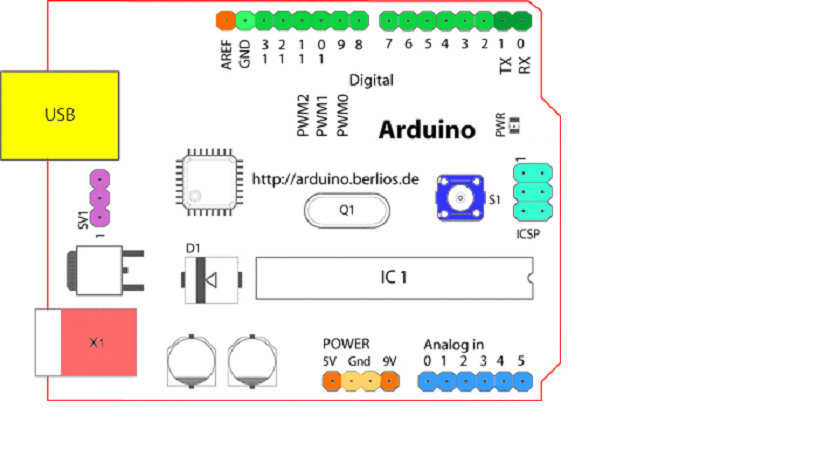
\includegraphics[scale=0.6]{AurdinoUNO.png}
\paragraph{•}
Starting clockwise from the top center: 
\begin{itemize}


\item Analog Reference pin (orange) 
\item Digital Ground (light green) 

\item Digital Pins 2-13 (green) 

\item Digital Pins 0-1/Serial In/Out - TX/RX (dark green) 

\item Reset Button - S1 (dark blue) 

\item In-circuit Serial Programmer (blue-green) 
\item Power and Ground Pins 
\item External Power Supply In (9-12VDC) - X1 (pink) 
\item External Power Supply In (9-12VDC) - X1 (pink) 
\item USB (used for uploading sketches to the board and for serial communication between the board and the computer; can be used to power the board) (yellow)
\end{itemize}
\subsubsection{Digital pins}
\paragraph{•}
\begin{description}
\item[$\bullet$ Serial: ] 0(RX) and 1(TX). Used to receive(RX)and transmit(TX) TTL serial data. On the Arduino Diecimila, these pins are connected to the corresponding pins of the FTDI USB-to-TTL Serial chip. On the Arduino BT, they are connected to the corresponding pins of the WT11 Bluetooth module. On the Arduino Mini and LilyPad Arduino, they are intended for use with an external TTL serial module (e.g. the Mini-USB Adapter). 
\end{description}

\begin{description}
\item[$\bullet$ External Interrupts :] 2 and 3. These pins can be configured to trigger an interrupt on a low value, a rising or falling edge, or a change in value.  
\end{description}
\begin{description}
\item[$\bullet$ PWM: ] 3, 5, 6, 9, 10, and 11. Provide 8-bit PWM output with the analogWrite() function. On boards with an ATmega8, PWM output is available only on pins 9, 10, and 11.  
\end{description}
\begin{description}
\item[$\bullet$ BT Reset: ] 7. (Arduino BT-only) Connected to the reset line of the bluetooth module.   
\end{description}
\begin{description}
\item[$\bullet$ SPI: ] 10 (SS), 11 (MOSI), 12 (MISO), 13 (SCK). These pins support SPI communication, which, although provided by the underlying hardware, is not currently included in the Arduino language. 
\end{description}

\begin{description}
\item[$\bullet$ LED:] 13. On the Diecimila and LilyPad, there is a built-in LED connected to digital pin 13. When the pin is HIGH value, the LED is on, when the pin is LOW, it's off. 
\end{description}

\subsubsection{Analog pins}
\paragraph{•}
In addition to the specific functions listed below, the analog input pins support 10-bit analog-to-digital conversion (ADC) using the analogRead() function. Most of the analog inputs can also be used as digital pins: analog input 0 as digital pin 14 through analog input 5 as digital pin 19. Analog inputs 6 and 7 (present on the Mini and BT) cannot be used as digital pins. 
\begin{description}
\item[$\bullet$ I2C:] 13. On the Diecimila and LilyPad, there is a built-in LED connected to digital pin 13. When the pin is HIGH value, the LED is on, when the pin is LOW, it's off. 
\end{description}
\subsubsection{Power pins}
\paragraph{•}
\begin{description}
\item[$\bullet$ VIN:] The input voltage to the Arduino board when it's using an external power source (as opposed to 5 volts from the USB connection or other regulated power source). You can supply voltage through this pin, or, if supplying voltage via the power jack, access it through this pin. Note that different boards accept different input voltages ranges, please see the documentation for your board. Also note that the LilyPad has no VIN pin and accepts only a regulated input. 
\end{description}
\begin{description}
\item[$\bullet$ 5V:] The regulated power supply used to power the microcontroller and other components on the board. This can come either from VIN via an on-board regulator, or be supplied by USB or another regulated 5V supply.  
\end{description}
\begin{description}
\item[$\bullet$ 3.3V] A 3.3 volt supply generated by the on-board FTDI chip. GND. Ground pins. 
\end{description}
\subsection{ESP8266-12E WiFi MODULE}
\begin{center}
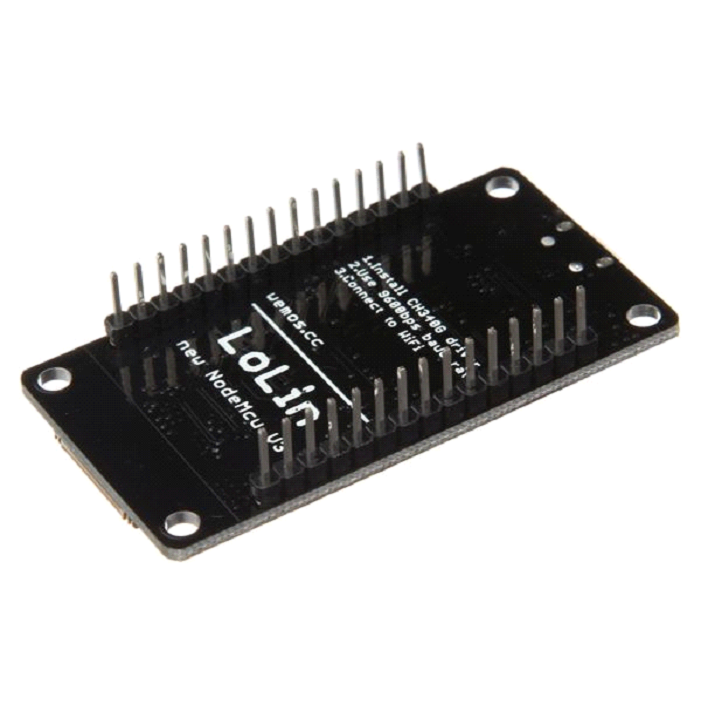
\includegraphics[scale=0.48]{wifi.png}
\end{center}
\paragraph{•}ESP-12E WiFi module is developed by Ai-thinker Team. core processor ESP8266 in smaller sizes of the module encapsulates Tensilica L106 integrates industry-leading ultra-low power 32-bit MCU micro, with the 16-bit short mode, Clock speed support 80 MHz, 160 MHz, supports the RTOS, integrated Wi-Fi MAC/BB/RF/PA/LNA, on-board antenna. The module supports standard IEEE802.11 b/g/n agreement, complete TCP/IP protocol stack. Users can use the add modules to an existing device networking, or building a separate network controller. ESP8266 is high integration wireless SOCs, designed for space and power constrained mobile platform designers. It provides unsurpassed ability to embed Wi-Fi capabilities within other systems, or to function as a standalone application, with the lowest cost, and minimal space requirement.
\paragraph{•}
ESP8266EX offers a complete and self-contained Wi-Fi networking solution; it can be used to host the application or to offload Wi-Fi networking functions from another application processor. When ESP8266EX hosts the application, it boots up directly from an external flash. Alternately, serving as a Wi-Fi adapter, wireless internet access can be added to any micro controller based design with simple connectivity (SPI/SDIO or I2C/UART interface).
\subsubsection{Features}
\begin{itemize}
\item 802.11 b/g/n
\item Integrated low power 32-bit MCU
\item Integrated 10-bit ADC
\item Integrated TCP/IP protocol stack
\item Integrated TR switch, balun, LNA, power amplifier and matching network
\item Integrated PLL, regulators, and power management units
\item Supports antenna diversity
\item Wi-Fi 2.4 GHz, support WPA/WPA2
\item Support STA/AP/STA+AP operation modes
\item Support Smart Link Function for both Android and iOS devices
\item Support Smart Link Function for both Android and iOS devices
\item Deep sleep power <10uA, Power down leakage current < 5uA
\item Wake up and transmit packets in < 2ms
\item Standby power consumption of < 1.0mW (DTIM3)
\item +20dBm output power in 802.11b mode
\item Operating temperature range -40C ~ 125C

\end{itemize}
\subsection{TEMPERATURE SENSOR LM35}
\begin{center}
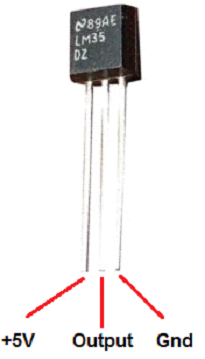
\includegraphics[scale=1]{temp.png}
\end{center}
\paragraph{As a temperature sensor, the circuit will read the temperature of the surrounding environment and relay this temperature to us back in degrees Celsius. The IC we used to measure the temperature is the LM35 IC integrated with the Arduino UNO to measure the temperature of the system. The Arduino UNO will then read this measured value from the LM35 (a low voltage IC, with 3 pins, uses approx. +5VDC) and translate into degrees Fahrenheit/Celsius, which we will be able to read from the computer from the Arduino serial monitor. 
}
\paragraph{The output pin provides an analog voltage output that is linearly proportional to the Celsius (Centigrade) temperature. Pin 2 gives an output of 1 millivolt per 0.1°C (10mV per degree). So to get the degree value in Celsius, all that must be done is to take the voltage output and divide it by 10- this give out the value degrees in Celsius. So, for example, if the output pin, pin 2, gives out a value of 315mV (0.315V), this is equivalent to a temperature of 31.5°C. 
}
\subsubsection{PINOUT DESCRIPTION}
\begin{center}
\begin{tabular}{ |c|c|c| }
\hline
\textbf{Pin No} & \textbf{Function} & \textbf{Name}\\
\hline
1 & Supply voltage; 5V (+35V to -2V) & VCC\\
\hline
2 & Output voltage (+6V to -1V) & Output\\
\hline
3 & Ground (0V) & Ground\\
\hline 
\end{tabular}
\end{center}


\end{document}